
%%% Local Variables:
%%% mode: latex
%%% TeX-master: t
%%% End:
\section{数据分析的``武器库''}

\begin{frame}{\textcolor{white}{空白}}

  \begin{columns}
    \begin{column}{.5\textwidth}
      \begin{figure}
        \centering 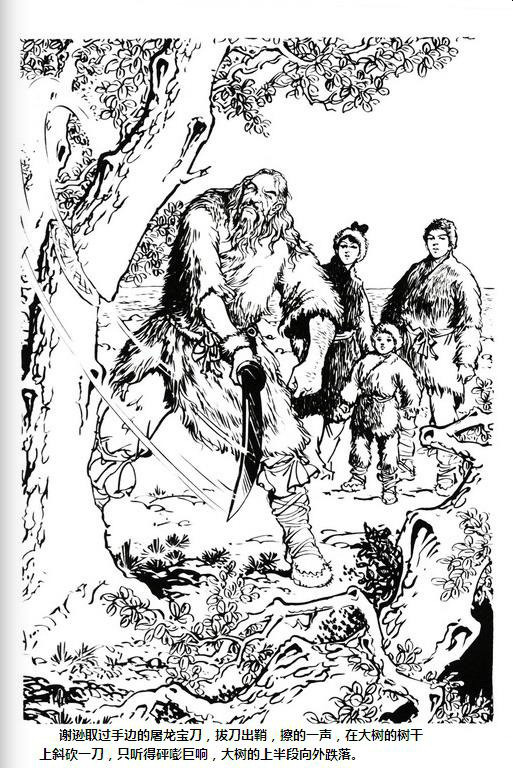
\includegraphics[width=0.95\columnwidth]{chp03_屠龙宝刀.jpg}
      \end{figure}
    \end{column}

    \begin{column}{.5\textwidth}
      \begin{ornamentblock}
        \centering
        {工欲善其事,必先利其器
          \rightline{\textemdash 《论语·卫灵公》}}
      \end{ornamentblock}
    \end{column}
  \end{columns}

\end{frame}

\begin{frame}{数据分析的``七种武器''}
\begin{enumerate}\large
\item 数据采集
\item 数据处理
\item 业务分析
\item 数据建模
\item 数据库
\item 分析算法
\item 可视化
\end{enumerate}
\end{frame}

\subsection{数据采集}
\begin{frame}[t]{\subsecname}
\begin{itemize}
\item<2-> 利用服务器端提供的API接口调取数据
\item<3-> 编写爬虫程序,从网页上抓取数据
\end{itemize}

\begin{overlayarea}{\textwidth}{\textheight}

  \begin{onlyenv}<2>
\begin{table} \centering \scriptsize
  \renewcommand\arraystretch{0.9}
  \begin{tabular}{|m{0.3\columnwidth}|m{0.3\columnwidth}|m{0.3\columnwidth}|}
    \toprule
    \rowcolor{LightCyan}
\multicolumn{1}{|c|}{\textbf{字段名称}} & \multicolumn{1}{c|}{\textbf{字段含义}} & \multicolumn{1}{c|}{\textbf{说明}}\\\hline
     alter & 交通出行方式 & 推荐公交、巴士优先、骑车、小汽车、出租车等 \\\hline
     O\_lon \& O\_lat & 出发地坐标 & 百度公司加密后的经纬度坐标 \\\hline
     D\_lon \& D\_lat & 到达地坐标 & 百度公司加密后的经纬度坐标 \\\hline
     distance & 出行距离 & 包括步行在内的实际路网距离\\\hline
     duration & 出行时间 & 包括步行在内 \\\hline
     price & 票价 & \\\hline
     walkDistance & 步行距离 & \\\hline
     walkTime & 步行时间 & \\\hline
     transferNumber & 换乘次数 & \\    
     \bottomrule
  \end{tabular}
\caption{百度地图API返回的公交路径规划数据结果}
\end{table}
  \end{onlyenv}

\vspace{-15pt}
  \begin{onlyenv}<3>
\begin{figure}
  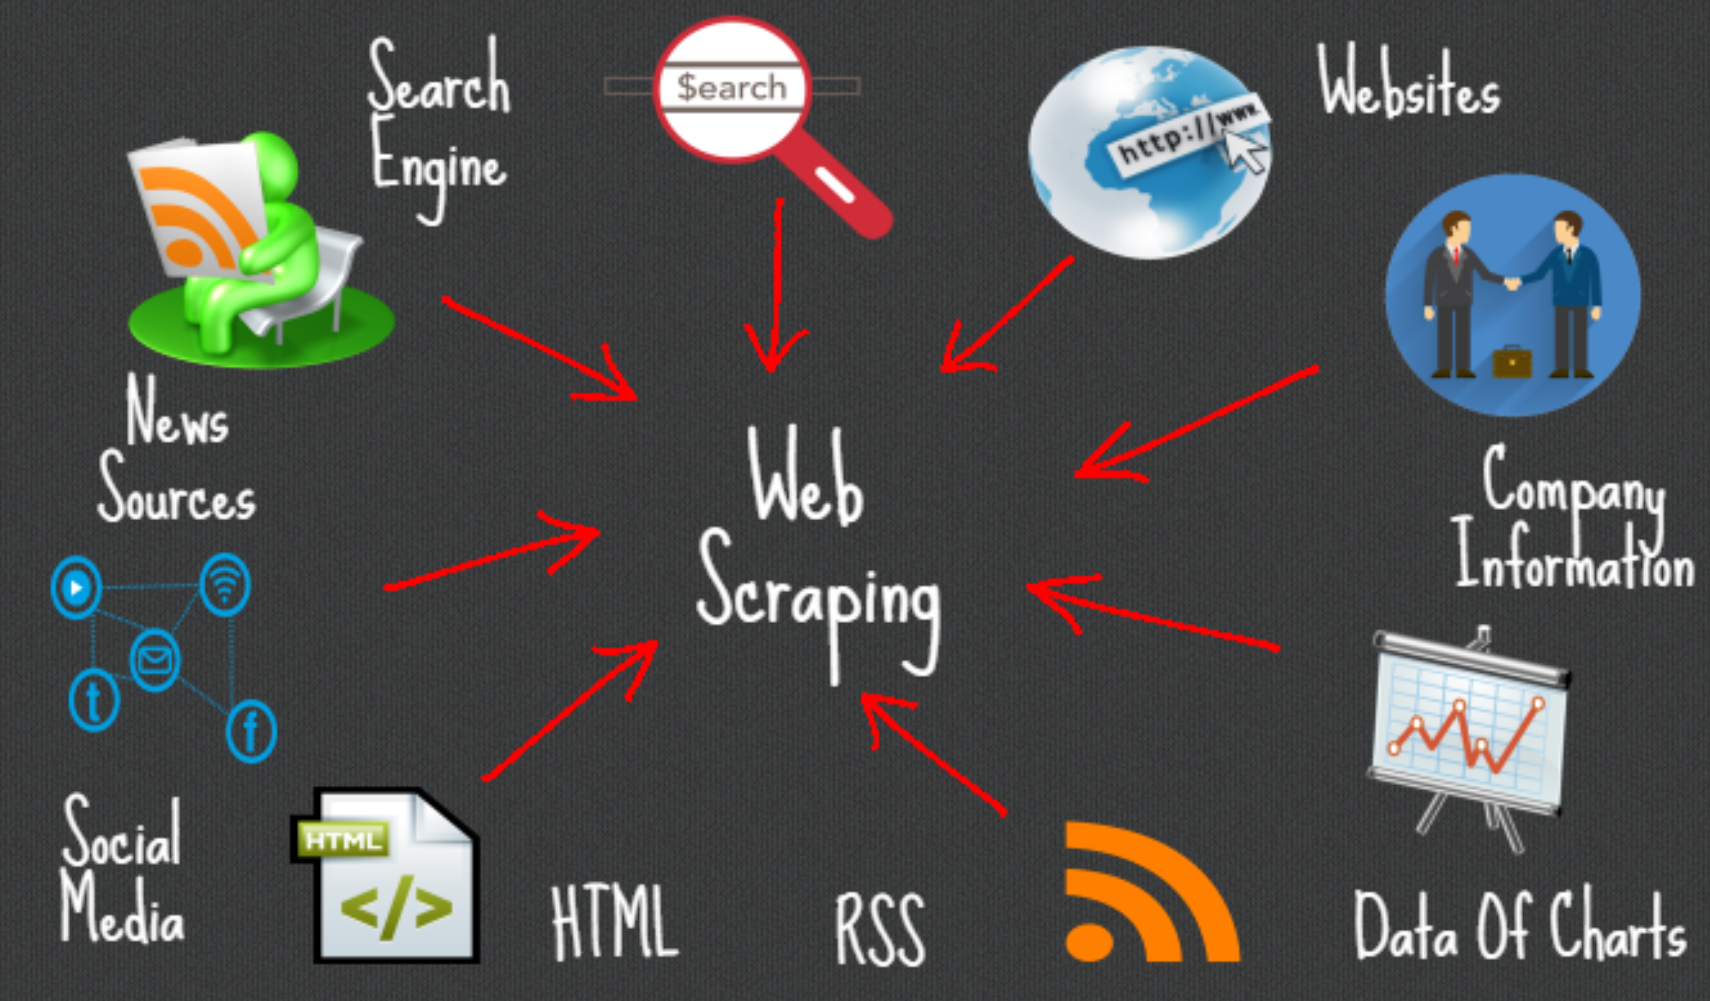
\includegraphics[width=\textwidth]{chp03_网络爬虫.png}
  \caption{利用爬虫程序,可以从丰富的互联网资源中自动化采集数据}
\end{figure}
  \end{onlyenv}
\end{overlayarea}

\end{frame}

\subsection{数据预处理}

\begin{frame}[t,fragile]{\subsecname}
\begin{itemize}
\item<1-> 现实中的原始数据都是不完整、不一致的脏数据,需要编写程序对数据进行\emphText{清洗、集成、变换和归约}等自动化处理
\item<2-> 示例:GPS数据预处理
\end{itemize}

\begin{overlayarea}{\textwidth}{\textheight}
  \begin{onlyenv}<2>
\begin{algorithm}[H] \tiny
     \SetKwInOut{Input}{输入}\SetKwInOut{Output}{输出}
     %\DontPrintSemicolon 
     \caption*{GPS原始数据清洗}
      
     \KwData{原始车牌GPS文件:GPS\_File,每行$line$=(ID,Postion,Time,Direction,Speed,State)}
     \KwResult{清洗后的GPS文件:GPS\_File\_P}
     \Input{时间容差$\Delta t$, 距离容差$\Delta d$,原始GPS数据列表$G$}
     \BlankLine

     \tcc{对$G$按照时间排序}
     SortByTime($G$)\;
     \BlankLine

     $bFirst$ $\leftarrow$ true\;

     \For{$i=1 \leftarrow 1$ \KwTo $N$}{
        \tcc{剔除位置不在市域范围$Rect$的错误点}
        \lIf{$G[i].position \notin Rect$}{\textbf{continue}}
           
        \eIf{$bFirst=true$}{
            GPS\_File\_P $\leftarrow$ OutputResult($G[i]$)\tcc*[r]{输出结果}
            $bFirst \leftarrow$ true; $tt \leftarrow G[i].time$; $tp \leftarrow G[i].position$;}
            {
            \tcc{根据前后点时间容差和距离容差剔除错误点}
            \If{$(5 \leqslant (G[i].time-tt) \leqslant{\Delta t}) \cap$
            Distance$(G[i].position,tp) \leqslant \Delta d$}
            {GPS\_File\_P $\leftarrow$ OutputResult($G[i]$)\tcc*[r]{输出结果} 
            $tt \leftarrow G[i].time$; $tp \leftarrow G[i].position$;}}
        }
\end{algorithm}
  \end{onlyenv}

  \begin{onlyenv}<3>
\begin{columns}
  \begin{column}{.4\textwidth}
\begin{figure}
  \centering
  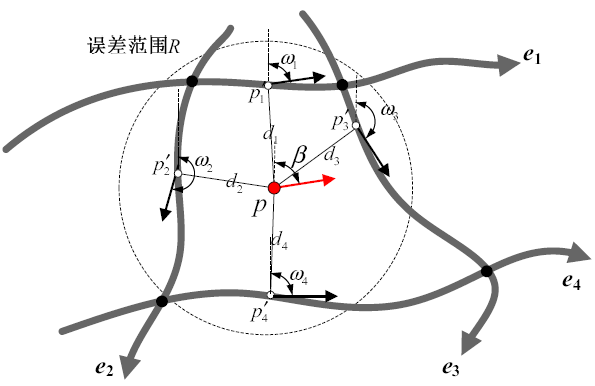
\includegraphics[width=\textwidth]{chp03_地图匹配示意.png}
\end{figure}
  \end{column}
  \begin{column}{.6\textwidth}
\begin{algorithm}[H] \tiny
     \SetKwInOut{Input}{输入}
     \SetKwInOut{Output}{输出}
     %\DontPrintSemicolon 
     \caption*{GPS与道路地图匹配}
     \Input{路网模型G和GPS轨迹$T$: $p_1 \rightarrow p_2 \rightarrow \cdots \rightarrow p_n$}
     \Output{处理后的GPS点序列$P$:$c_1^{j_1} \rightarrow c_2^{j_2} \rightarrow \cdots c_n^{j_n}$}
     \BlankLine    
     \tcc{清空列表$tList$}
     $tList \leftarrow empty$\; 
     \For{$i = 1$ \KwTo $n$}{
       \tcc{误差范围R内的候选路段集}
       $s$ = GetCandidates($p_i$,$G$,$R$)\; 
       $tList.add(s)$\;}
     $G_T^{\prime}$ = ConstructGraph($tList$)\tcc*[r]{构建图$G_T^{\prime}$}
     \Return FindMatchedSequence($G_T^{\prime}$)\;
\end{algorithm}
  \end{column}
\end{columns}
  \end{onlyenv}
\end{overlayarea}
\end{frame}

\subsection{业务分析}

\begin{frame}[t]{\subsecname}
\begin{itemize}
\item 数据分析中\emphText{最关键的环节}
\item 结合业务特点,确定待分析的内容和技术路线
\end{itemize}

\begin{figure}
  \centering
  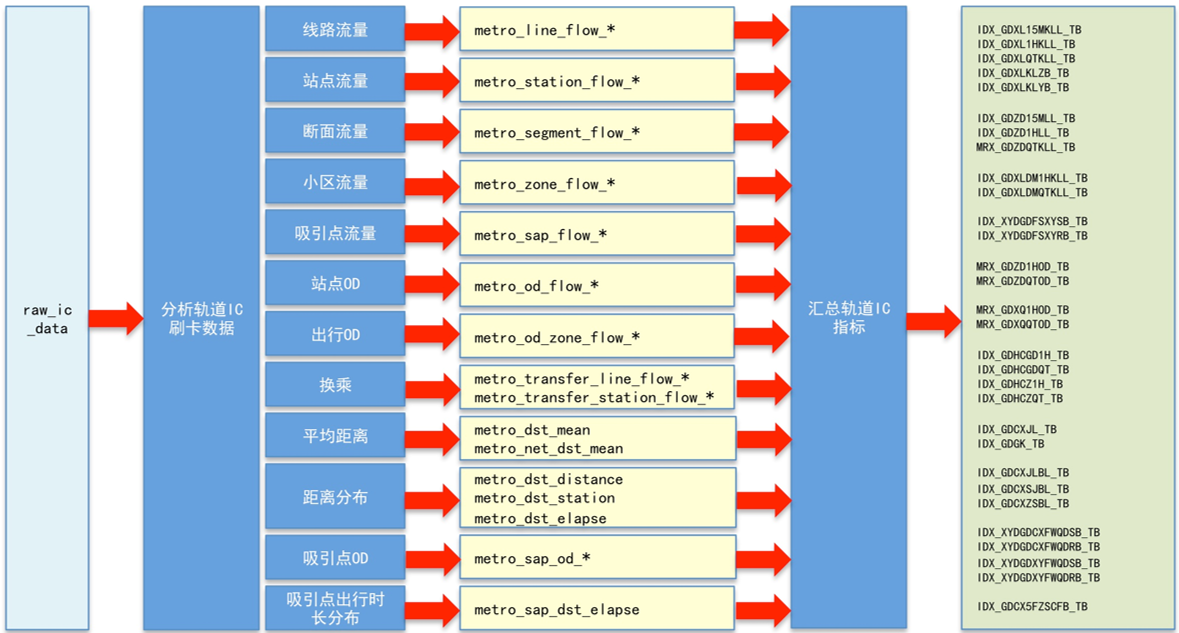
\includegraphics[width=\textwidth]{chp03_轨道刷卡业务分析.png}
  \caption{轨道刷卡数据分析的业务流程}
\end{figure}
\end{frame}

\subsection{数据建模}

\begin{frame}[t]{\subsecname}
\begin{itemize}
\item<1-> \emphText{根据业务需求对数据进行抽象},形成计算机能够理解的逻辑关系和物理结构
\item<2-> 示例:车辆轨迹模型 
\end{itemize}

\begin{overlayarea}{\textwidth}{\textheight}
  \begin{onlyenv}<2>
\begin{figure}
  \centering
  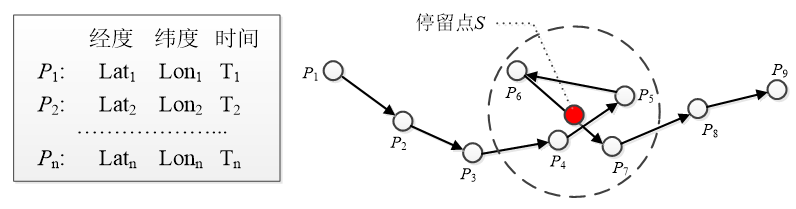
\includegraphics[width=0.8\textwidth]{chp03_停靠点提取算法.png} \\
  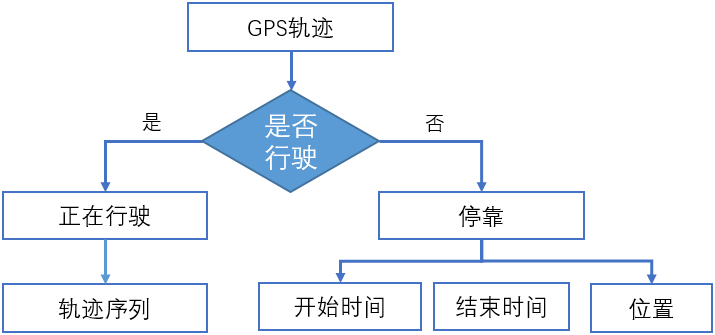
\includegraphics[width=0.6\textwidth]{chp03_GPS轨迹模型.png}
  \caption{车辆轨迹模型}
\end{figure}
  \end{onlyenv}
\end{overlayarea}
\end{frame}

\subsection{数据库}
\begin{frame}[t]{\subsecname}
\begin{itemize}
\item<1-> 通过高效的组织和存储,实现数据“增删改查”操作
\item<2-> 根据数据量级、数据内容、应用场景选择最适合的数据库技术
\item<3-> 数据库是大数据最核心的技术之一,目前主流采用\emphText{分布式存储方案}来解决
\end{itemize}

\begin{overlayarea}{\textwidth}{\textheight}
\vspace{-5pt}
  \begin{onlyenv}<1>
\begin{figure} \centering
\begin{columns}[b]
  \begin{column}{.5\textwidth}
    \begin{figure}
      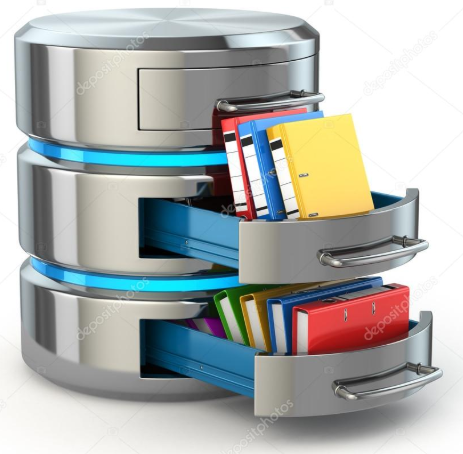
\includegraphics[height=0.4\textheight]{chp03_数据库技术1.png}
    \end{figure}
  \end{column}
  \begin{column}{.5\textwidth}
    \begin{figure}\flushleft
      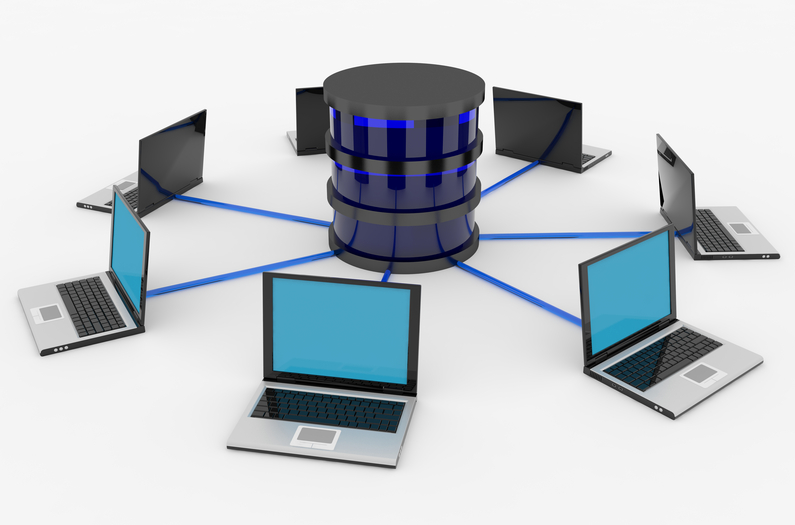
\includegraphics[height=0.35\textheight]{chp03_数据库技术2.png}
    \end{figure}
  \end{column}
\end{columns}
\caption{数据库技术的核心是对数据进行高效组织存储,以及多终端并发查询访问} 
\end{figure}
  \end{onlyenv}

\vspace{-10pt}
  \begin{onlyenv}<2>
\begin{figure}
  \centering
  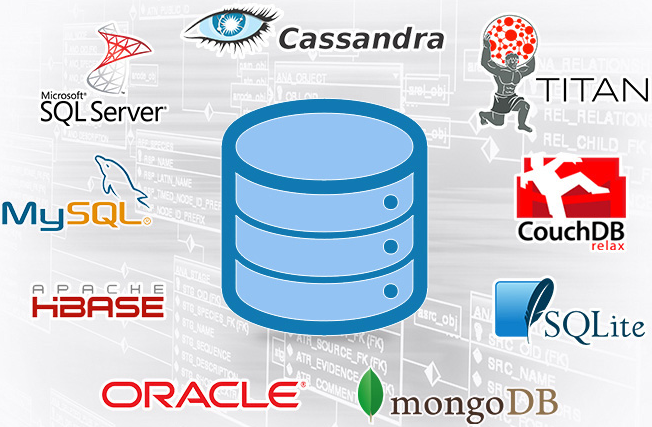
\includegraphics[width=0.7\textwidth]{chp03_数据库选择.png}
  \caption{根据实际需求选择最合适的数据库}
\end{figure}
  \end{onlyenv}

  \begin{onlyenv}<3>
\begin{figure}
  \centering
  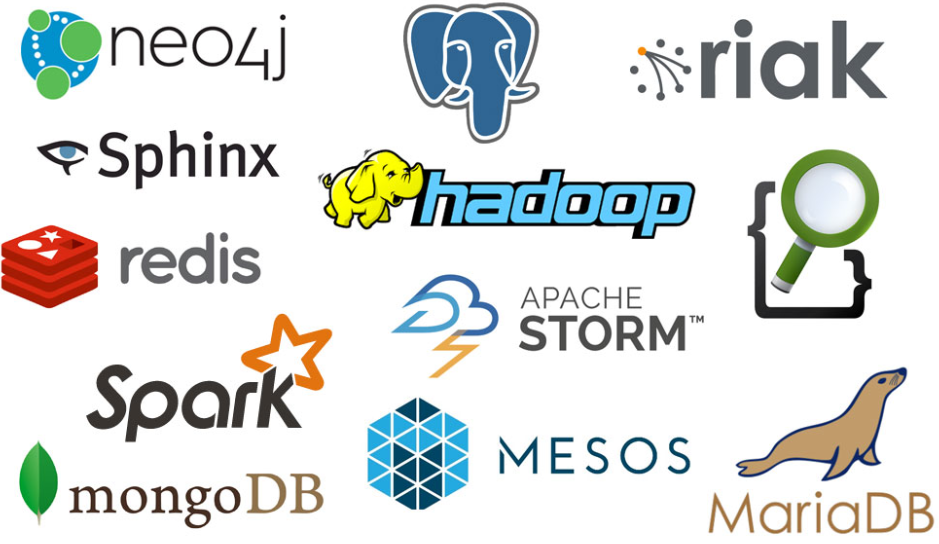
\includegraphics[width=0.8\textwidth]{chp03_大数据数据库产品.png}
  \caption{目前主流的大数据数据库产品}
\end{figure}
  \end{onlyenv}
\end{overlayarea}
\end{frame}

\subsection{分析算法}
\begin{frame}[t]{\subsecname}
\begin{itemize}
\item<1-> 算法不是简单的统计,而要能挖掘数据的规律和关系
\item<2-> 交通规划中最常用的分析算法是\emphText{空间分析算法}
\item<3-> 示例:核密度分析
\end{itemize}

\begin{overlayarea}{\textwidth}{\textheight}
  \begin{onlyenv}<3>
\begin{figure}
  \centering
  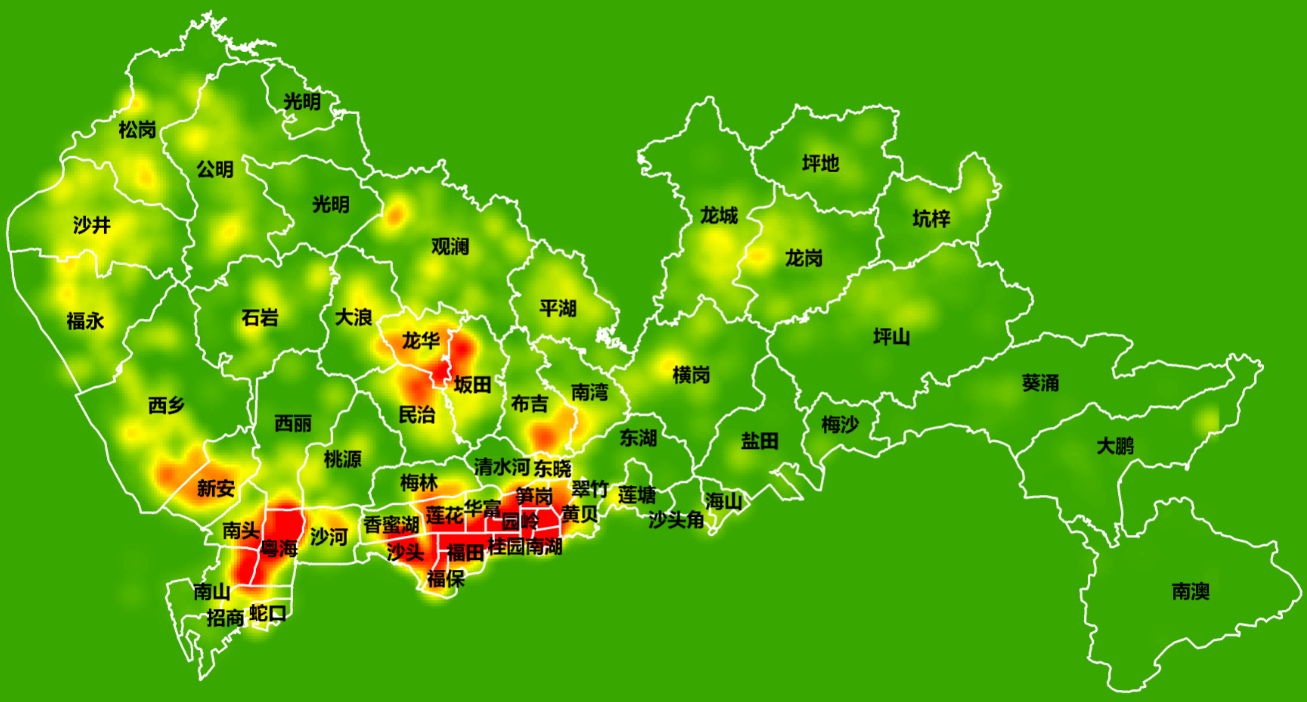
\includegraphics[width=0.9\textwidth]{chp03_核密度分析.png}
  \caption{核密度分析}
\end{figure}
  \end{onlyenv}

\vspace{-5pt}
\only<4>{
    \begin{columns}[c]
      \begin{column}{0.4\textwidth}
         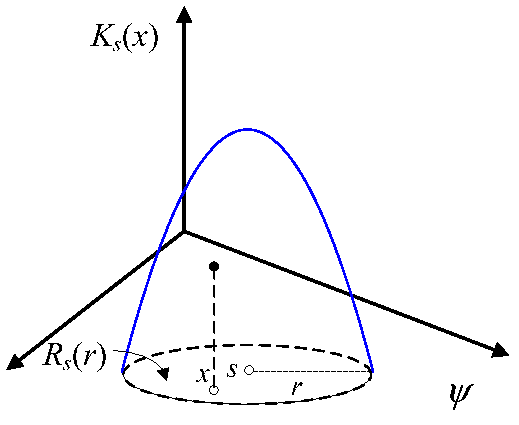
\includegraphics[width=1\columnwidth]{chp03_KDE模型.pdf}
      \end{column}

      \begin{column}{0.6\textwidth}
         \begin{beamerboxesrounded}{\small 带权重的核密度估计 \footnotemark[1]$^,$\footnotemark[2]}\scriptsize
           \[\hat \lambda (s) = \frac{1}{{n\pi {r^2}}}\sum\nolimits_{i = 1}^n {{w_i}{K_s}\left( {\frac{{{d_{sx}}}}{r}} \right)}\]
           其中,${d_{sx}} = \left\| {s - {x_i}} \right\|$表示位置$s$和第$i$个样本$x_i$之间的欧式距离;$r$被称为带宽,表示区域${R_s}(r)$的面积大小。
         \end{beamerboxesrounded}
      \end{column}
    \end{columns}

    \begin{itemize} \tiny
      \item KDE的核心思想就是通过计算单位面积内样本的核密度平滑处理来估计位置的属性值
      \item KDE结果表示区域${R_s}(r)$内不同样本对估计$s$ 位置属性值的权重
      \item 核函数是一个与距离有关的函数,而且其赋予区域${R_s}(r)$内每个样本点的值是不同的,离中心位置$s$ 越远的样本点,其值应该越小,而离中心位置$s$越近的样本点,其值应该越大
      \item 对KDE结果产生影响的两个因素包括核函数的形式以及带宽的选择
    \end{itemize}

\vspace{5pt}
    \footnotetext[1]{\tiny Silverman B W. 1986. Density Estimation for Statistics and Data Analysis[M]. London: Chapman Hall.}
    \footnotetext[2]{\tiny Wand M P, Jones M C. 1995. Kernel Smoothing[M]. Boca Raton, Florida: Chapman \& Hall/CRC. }}

\vspace{-10pt}
\only<5>{
   \begin{figure}
       \subfloat[Uniform]
           {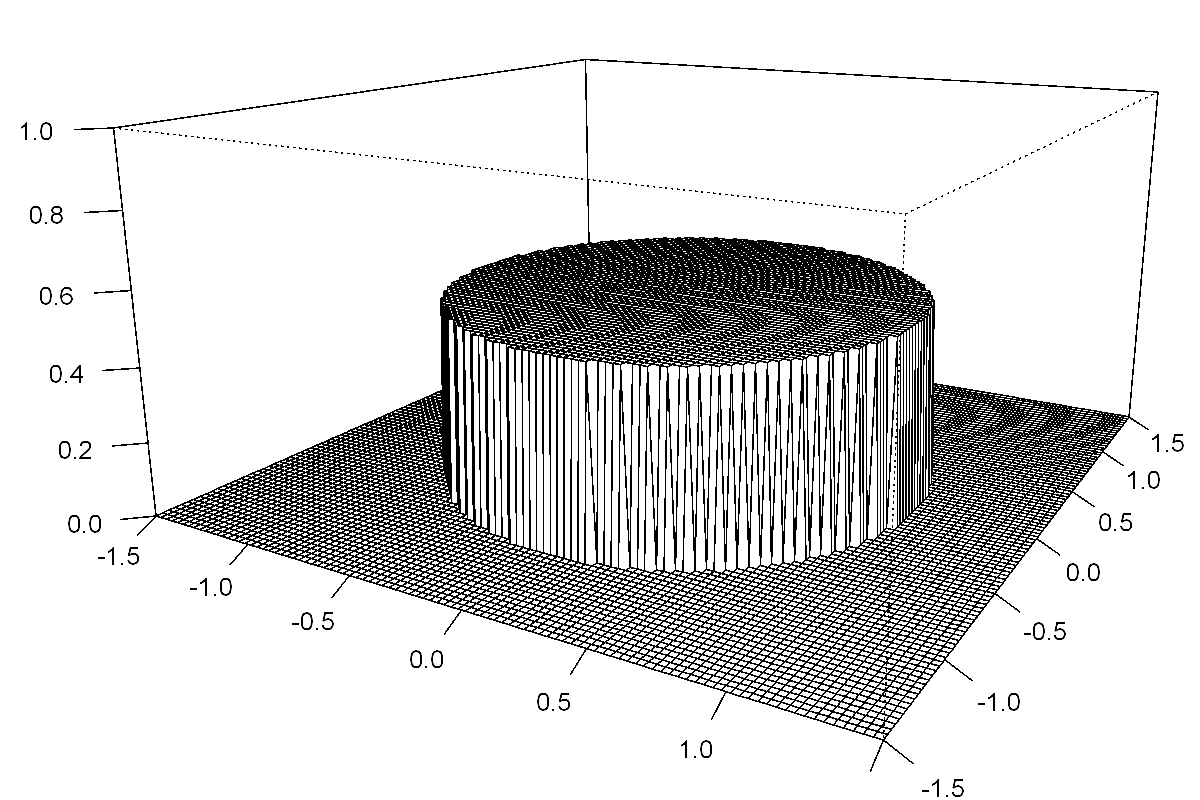
\includegraphics[width=0.24\columnwidth]
           {chp03_Function_Uniform.pdf}}\vspace{0.5pt}
       \subfloat[Triangular]
           {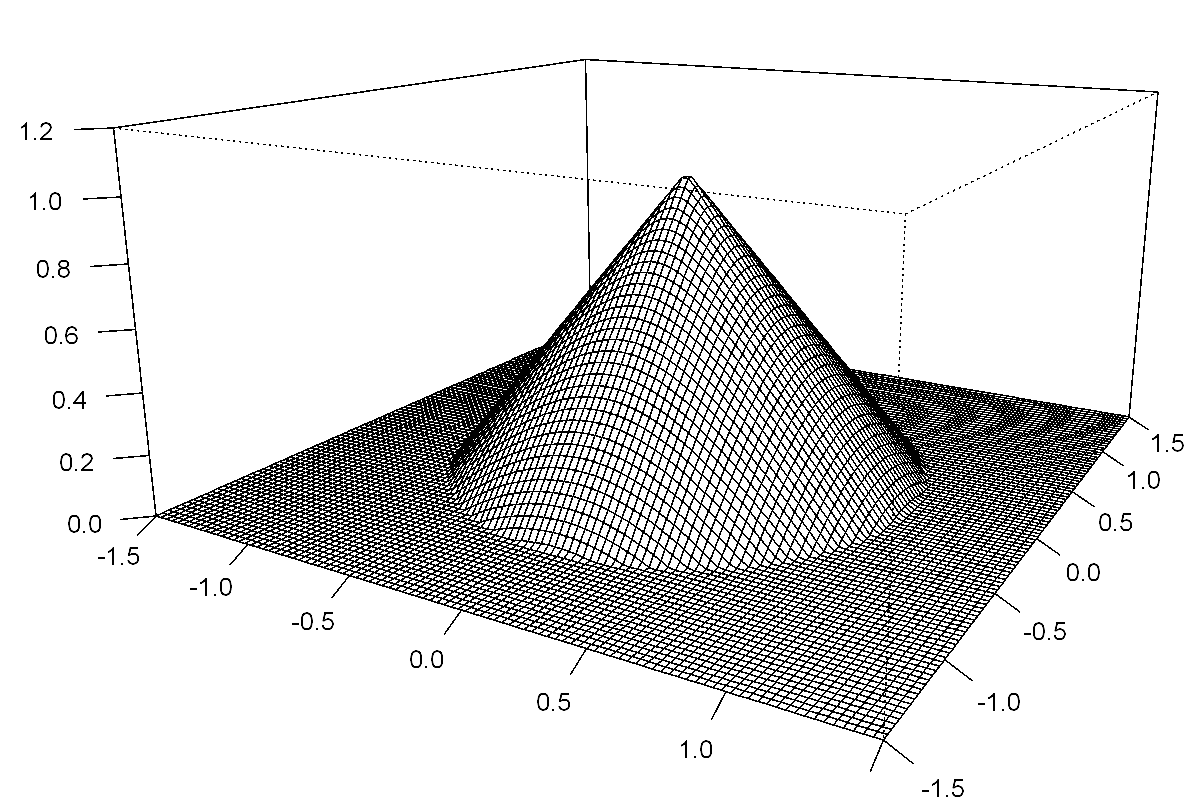
\includegraphics[width=0.24\columnwidth]
           {chp03_Function_Triangular.pdf}}\vspace{0.5pt}
       \subfloat[Quartic]
           {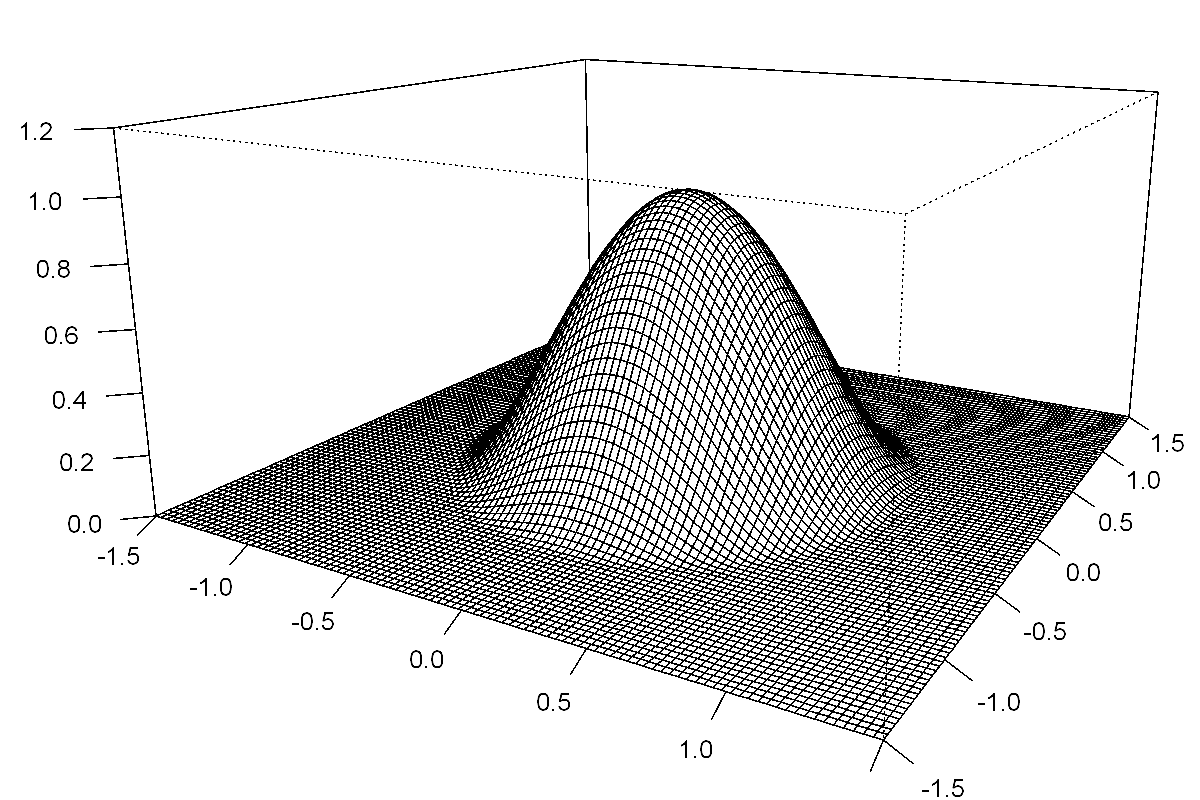
\includegraphics[width=0.24\columnwidth]
           {chp03_Function_Quartic.pdf}} \vspace{0.5pt}
       \subfloat[Triweight]
           {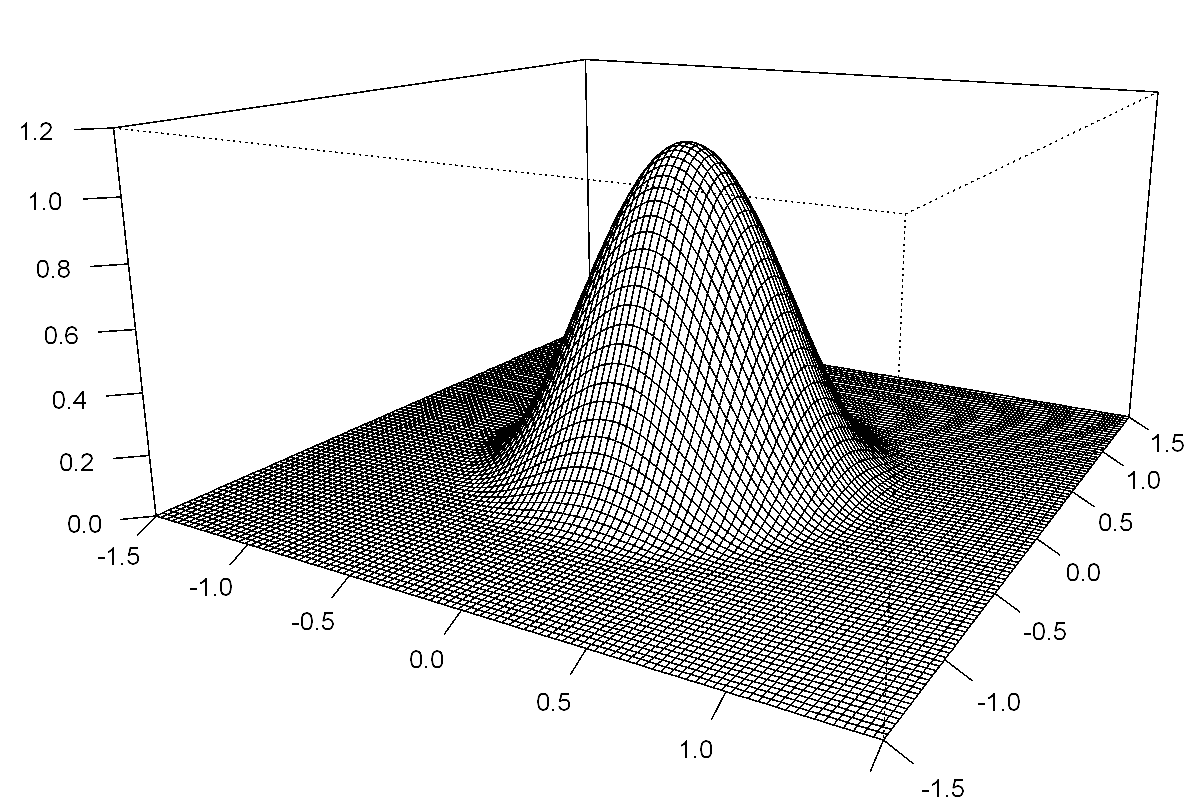
\includegraphics[width=0.24\columnwidth]
           {chp03_Function_Triweight.pdf}} \\
       \subfloat[Tricube]
           {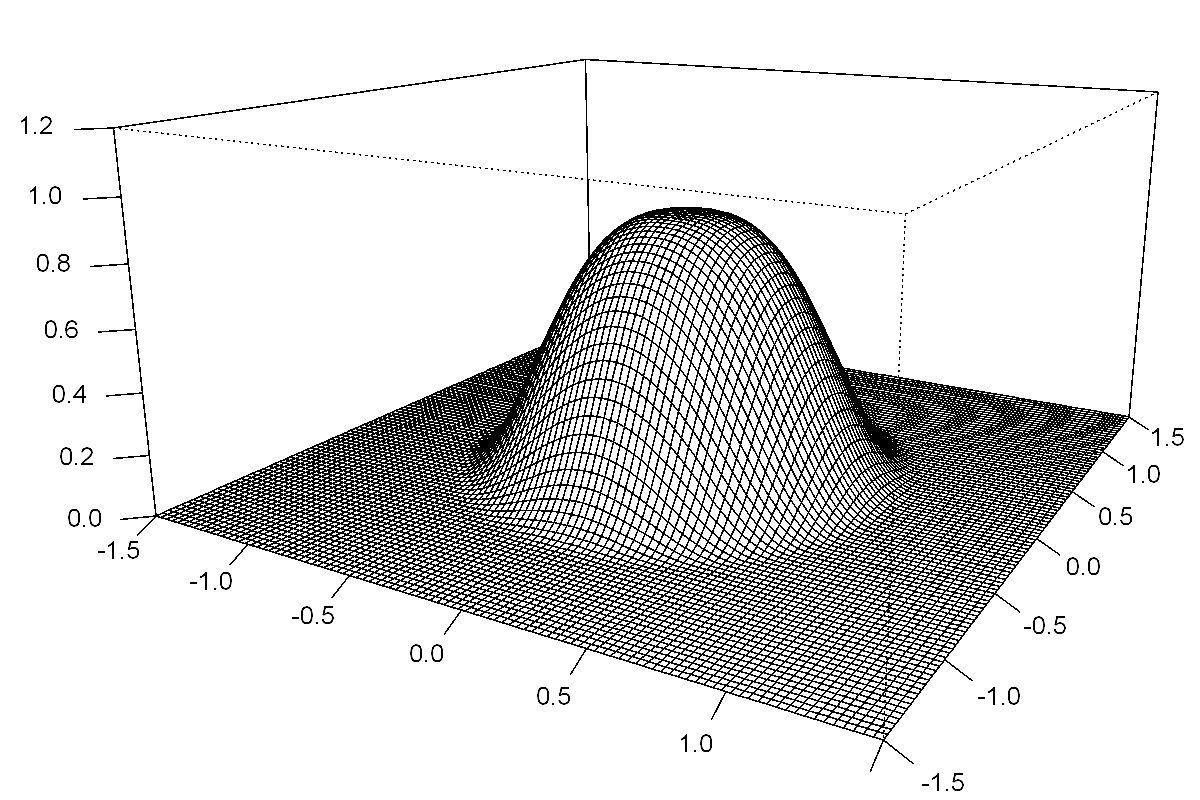
\includegraphics[width=0.24\columnwidth]
           {chp03_Function_Tricube.pdf}}  \vspace{0.5pt}
       \subfloat[Epanechnikov]
           {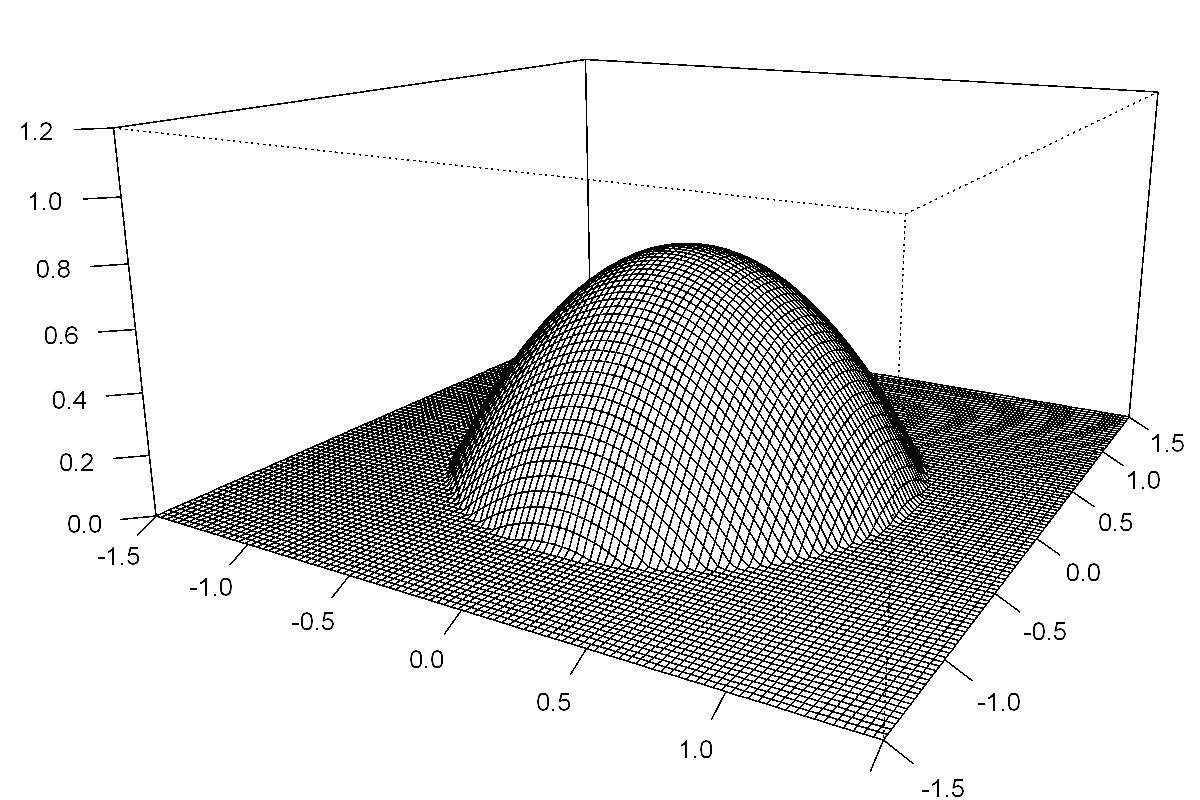
\includegraphics[width=0.24\columnwidth]
           {chp03_Function_Epanechnikov.pdf}} \vspace{0.5pt}
       \subfloat[Gaussian]
           {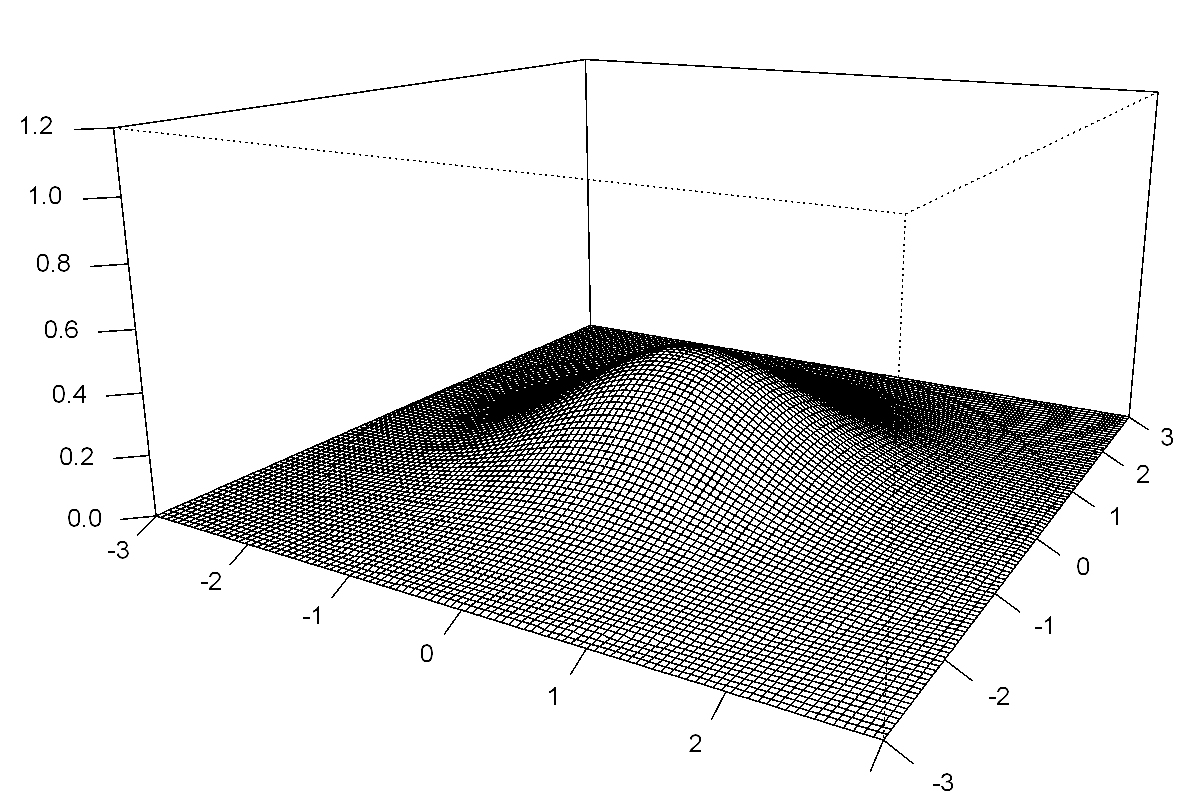
\includegraphics[width=0.24\columnwidth]
           {chp03_Function_Gaussian.pdf}}   \vspace{0.5pt}
       \caption{常见的核函数}
   \end{figure}}
\end{overlayarea}
\end{frame}

\subsection{可视化}
\begin{frame}[t]{\subsecname}
\begin{itemize}
\item<1-> 计算机技术与艺术的结合
\item<2-> \emphText{将绘图与数据分离,数据相关绘图与数据无关绘图分离}
\item<3-> 示例:变形地图(cartogram)
\end{itemize}

\begin{overlayarea}{\textwidth}{\textheight}
  \begin{onlyenv}<1>
  \begin{columns}
    \begin{column}{.4\textwidth}
      \begin{figure}
        \centering 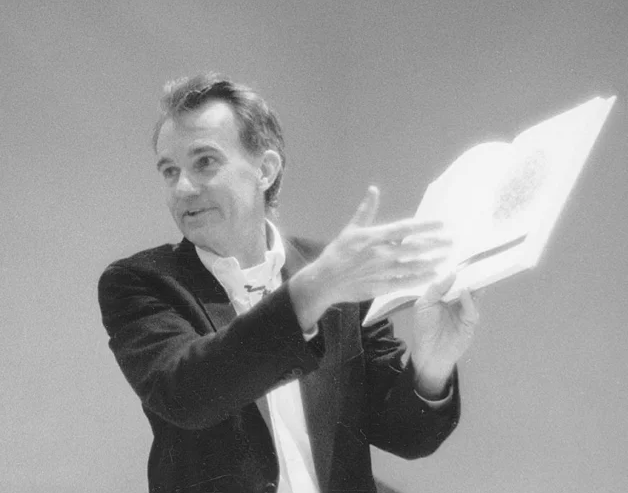
\includegraphics[width=\columnwidth]{chp03_edward_tufte.png}
        \caption{\scriptsize Edward Tufte(1942-),美国统计学家,数据可视化理论的先驱者和领军人物,人称“数据
    达芬奇”}
      \end{figure}
    \end{column}

    \begin{column}{.6\textwidth}
  \begin{ornamentblock}
    {The commonality between science and art is in trying to see profoundly - to develop strategies of seeing and showing.\\
      \rightline{\textemdash Edward Tufte}}
  \end{ornamentblock}
    \end{column}
  \end{columns}
  \end{onlyenv}

\vspace{-10pt}
  \begin{onlyenv}<2>
\begin{figure}[ht]
  \centering
  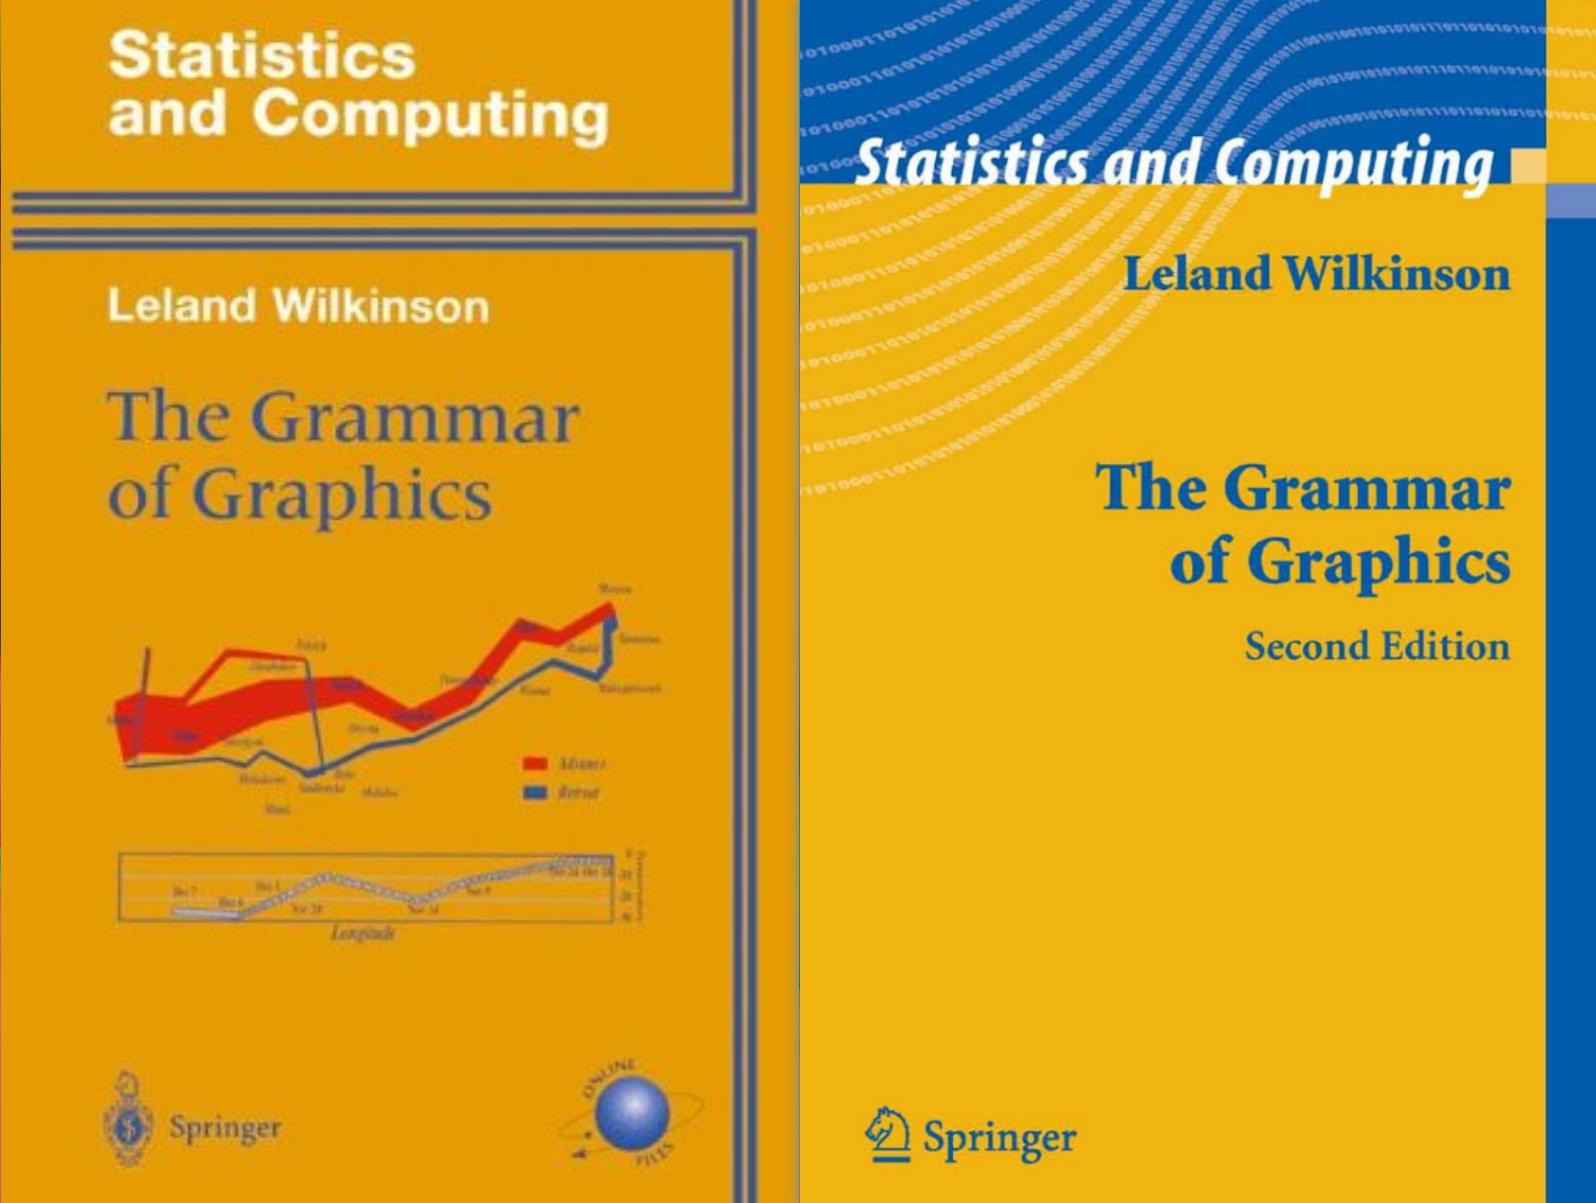
\includegraphics[width=0.65\columnwidth]{chp03_the_grammar_of_graphics.png}
  \caption{可视化领域经典著作《The Grammar of Graphics》的第一版(1999)和第二版(2005)}
\end{figure}
  \end{onlyenv}

\vspace{-10pt}
  \begin{onlyenv}<3>
\begin{figure}
  \centering
  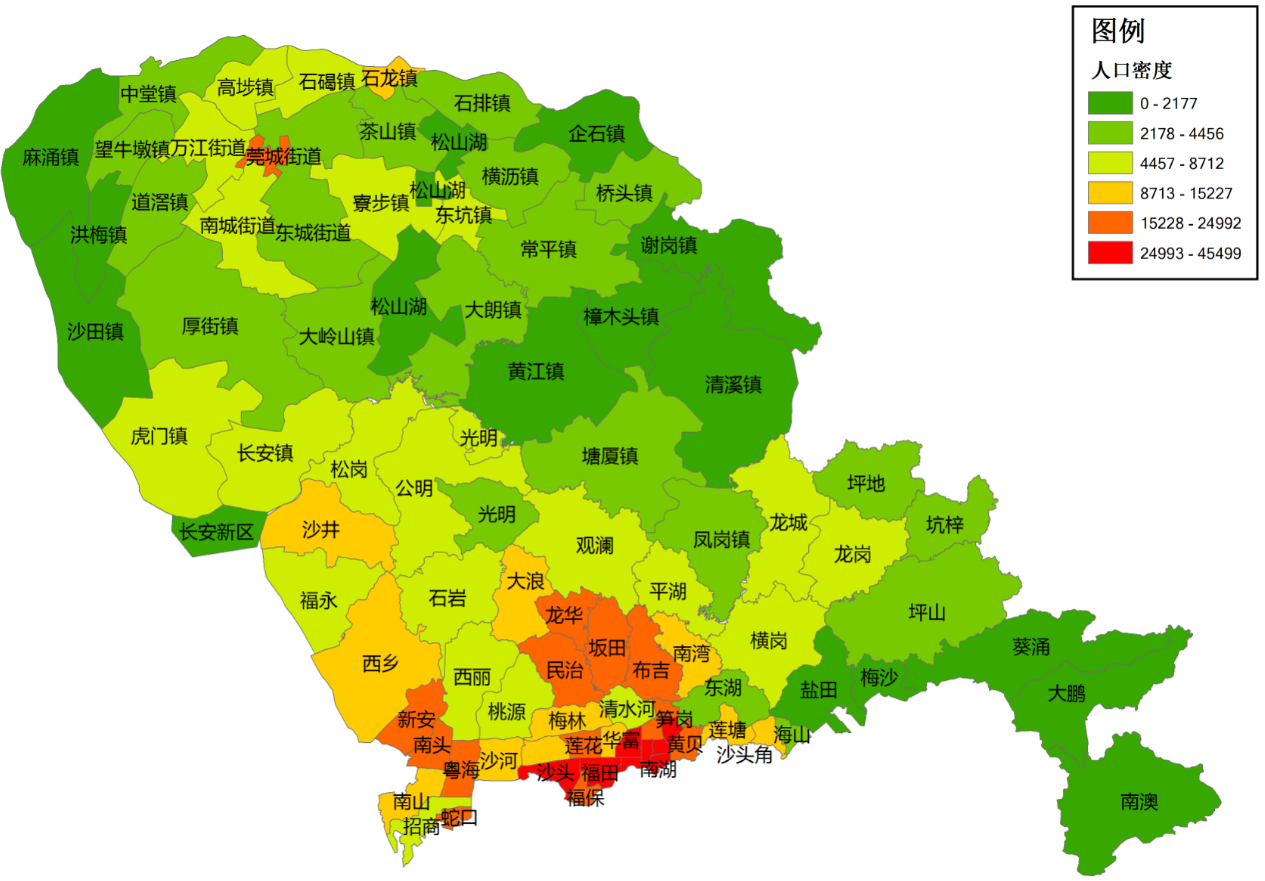
\includegraphics[width=0.8\textwidth]{chp04_人口.png}
  \caption{深莞街道人口密度}
\end{figure}
  \end{onlyenv}

  \begin{onlyenv}<4>
\begin{figure}
  \centering
  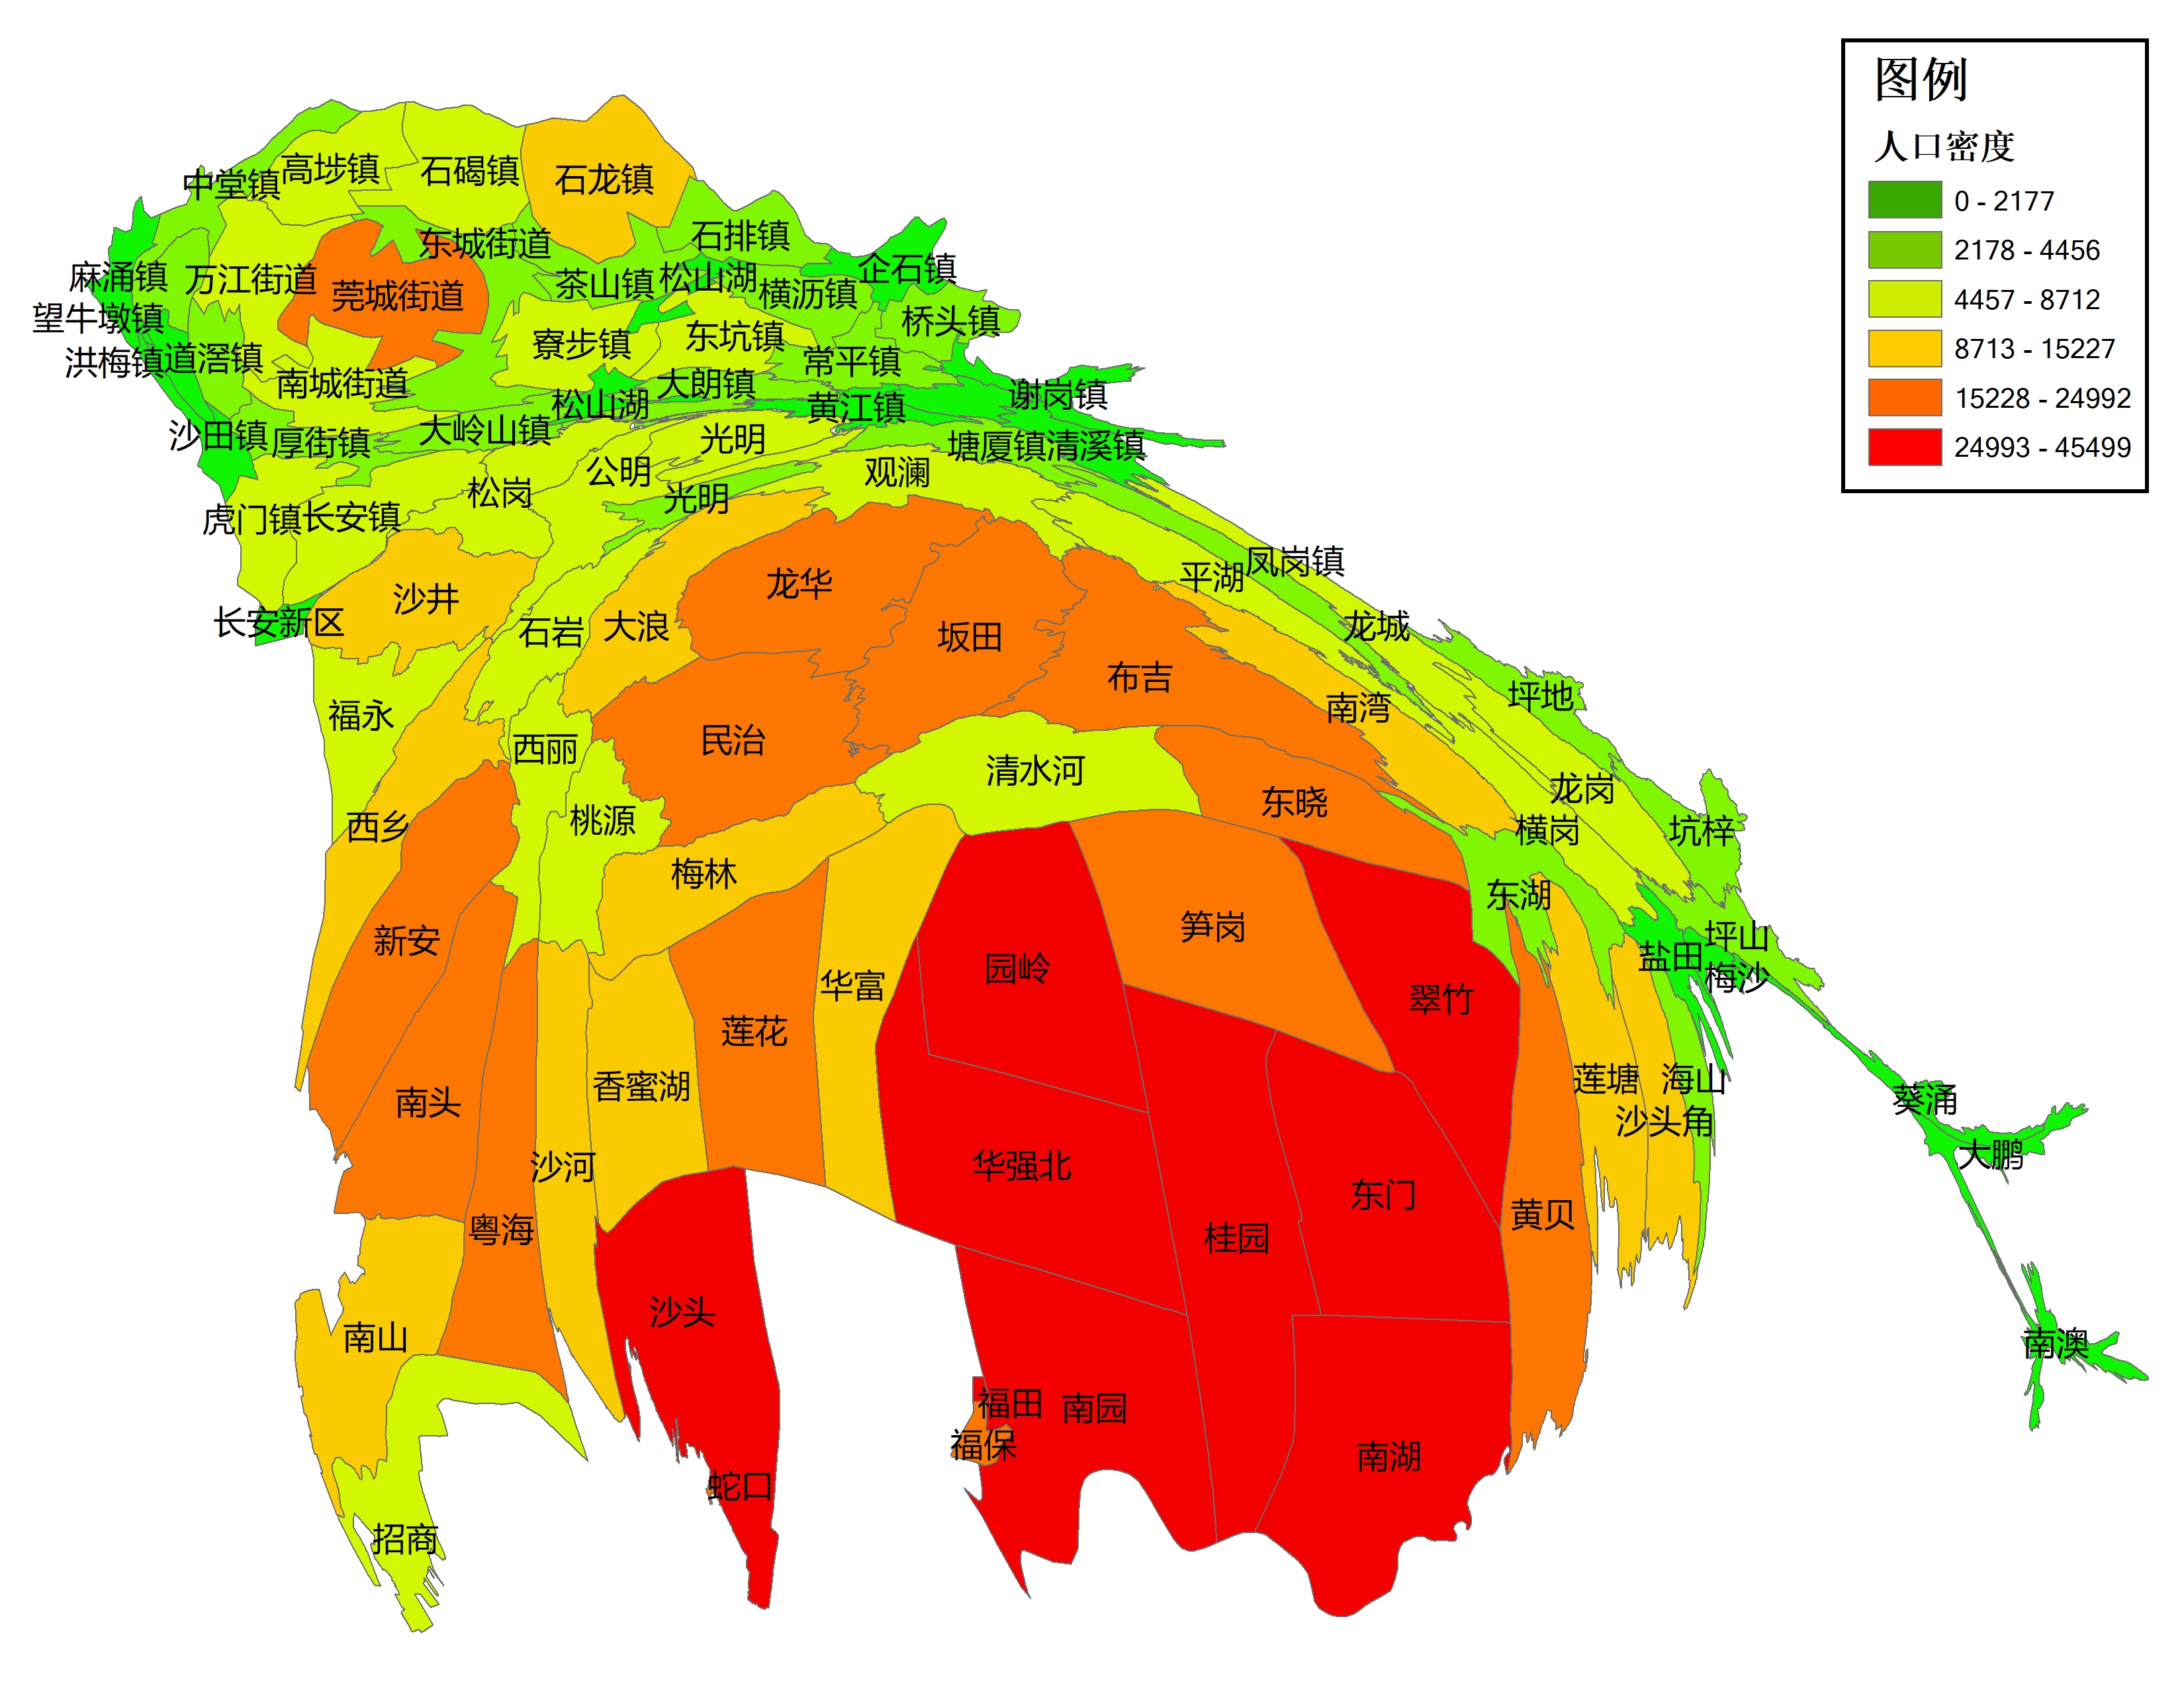
\includegraphics[width=0.7\textwidth]{chp04_人口密度cartogram.jpg}
  \caption{深莞街道人口密度变形地图(cartogram)}
\end{figure}
  \end{onlyenv}

  \begin{onlyenv}<5>
\begin{figure}
  \centering
  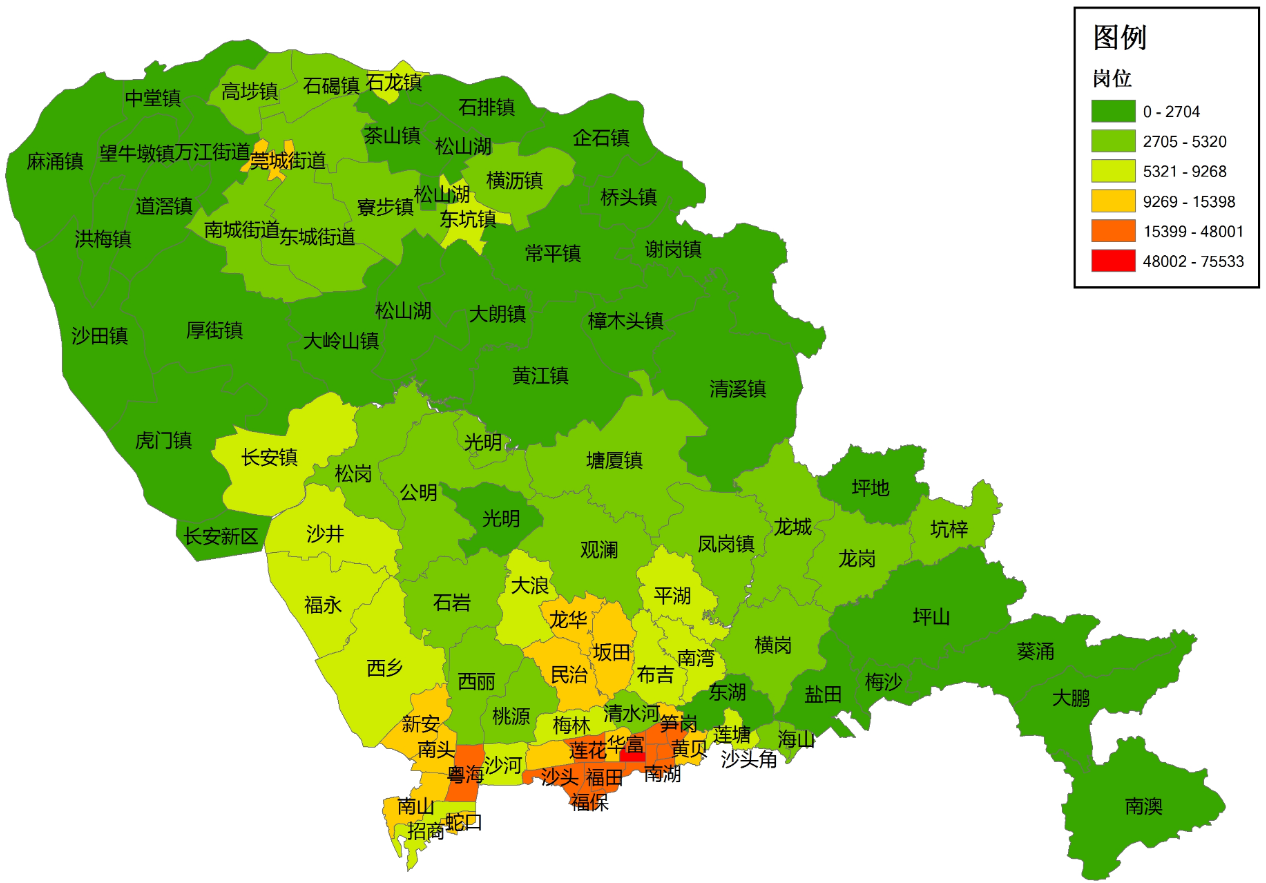
\includegraphics[width=0.8\textwidth]{chp04_岗位.png}
  \caption{深莞街道岗位密度}
\end{figure}
  \end{onlyenv}

  \begin{onlyenv}<6>
\begin{figure}
  \centering
  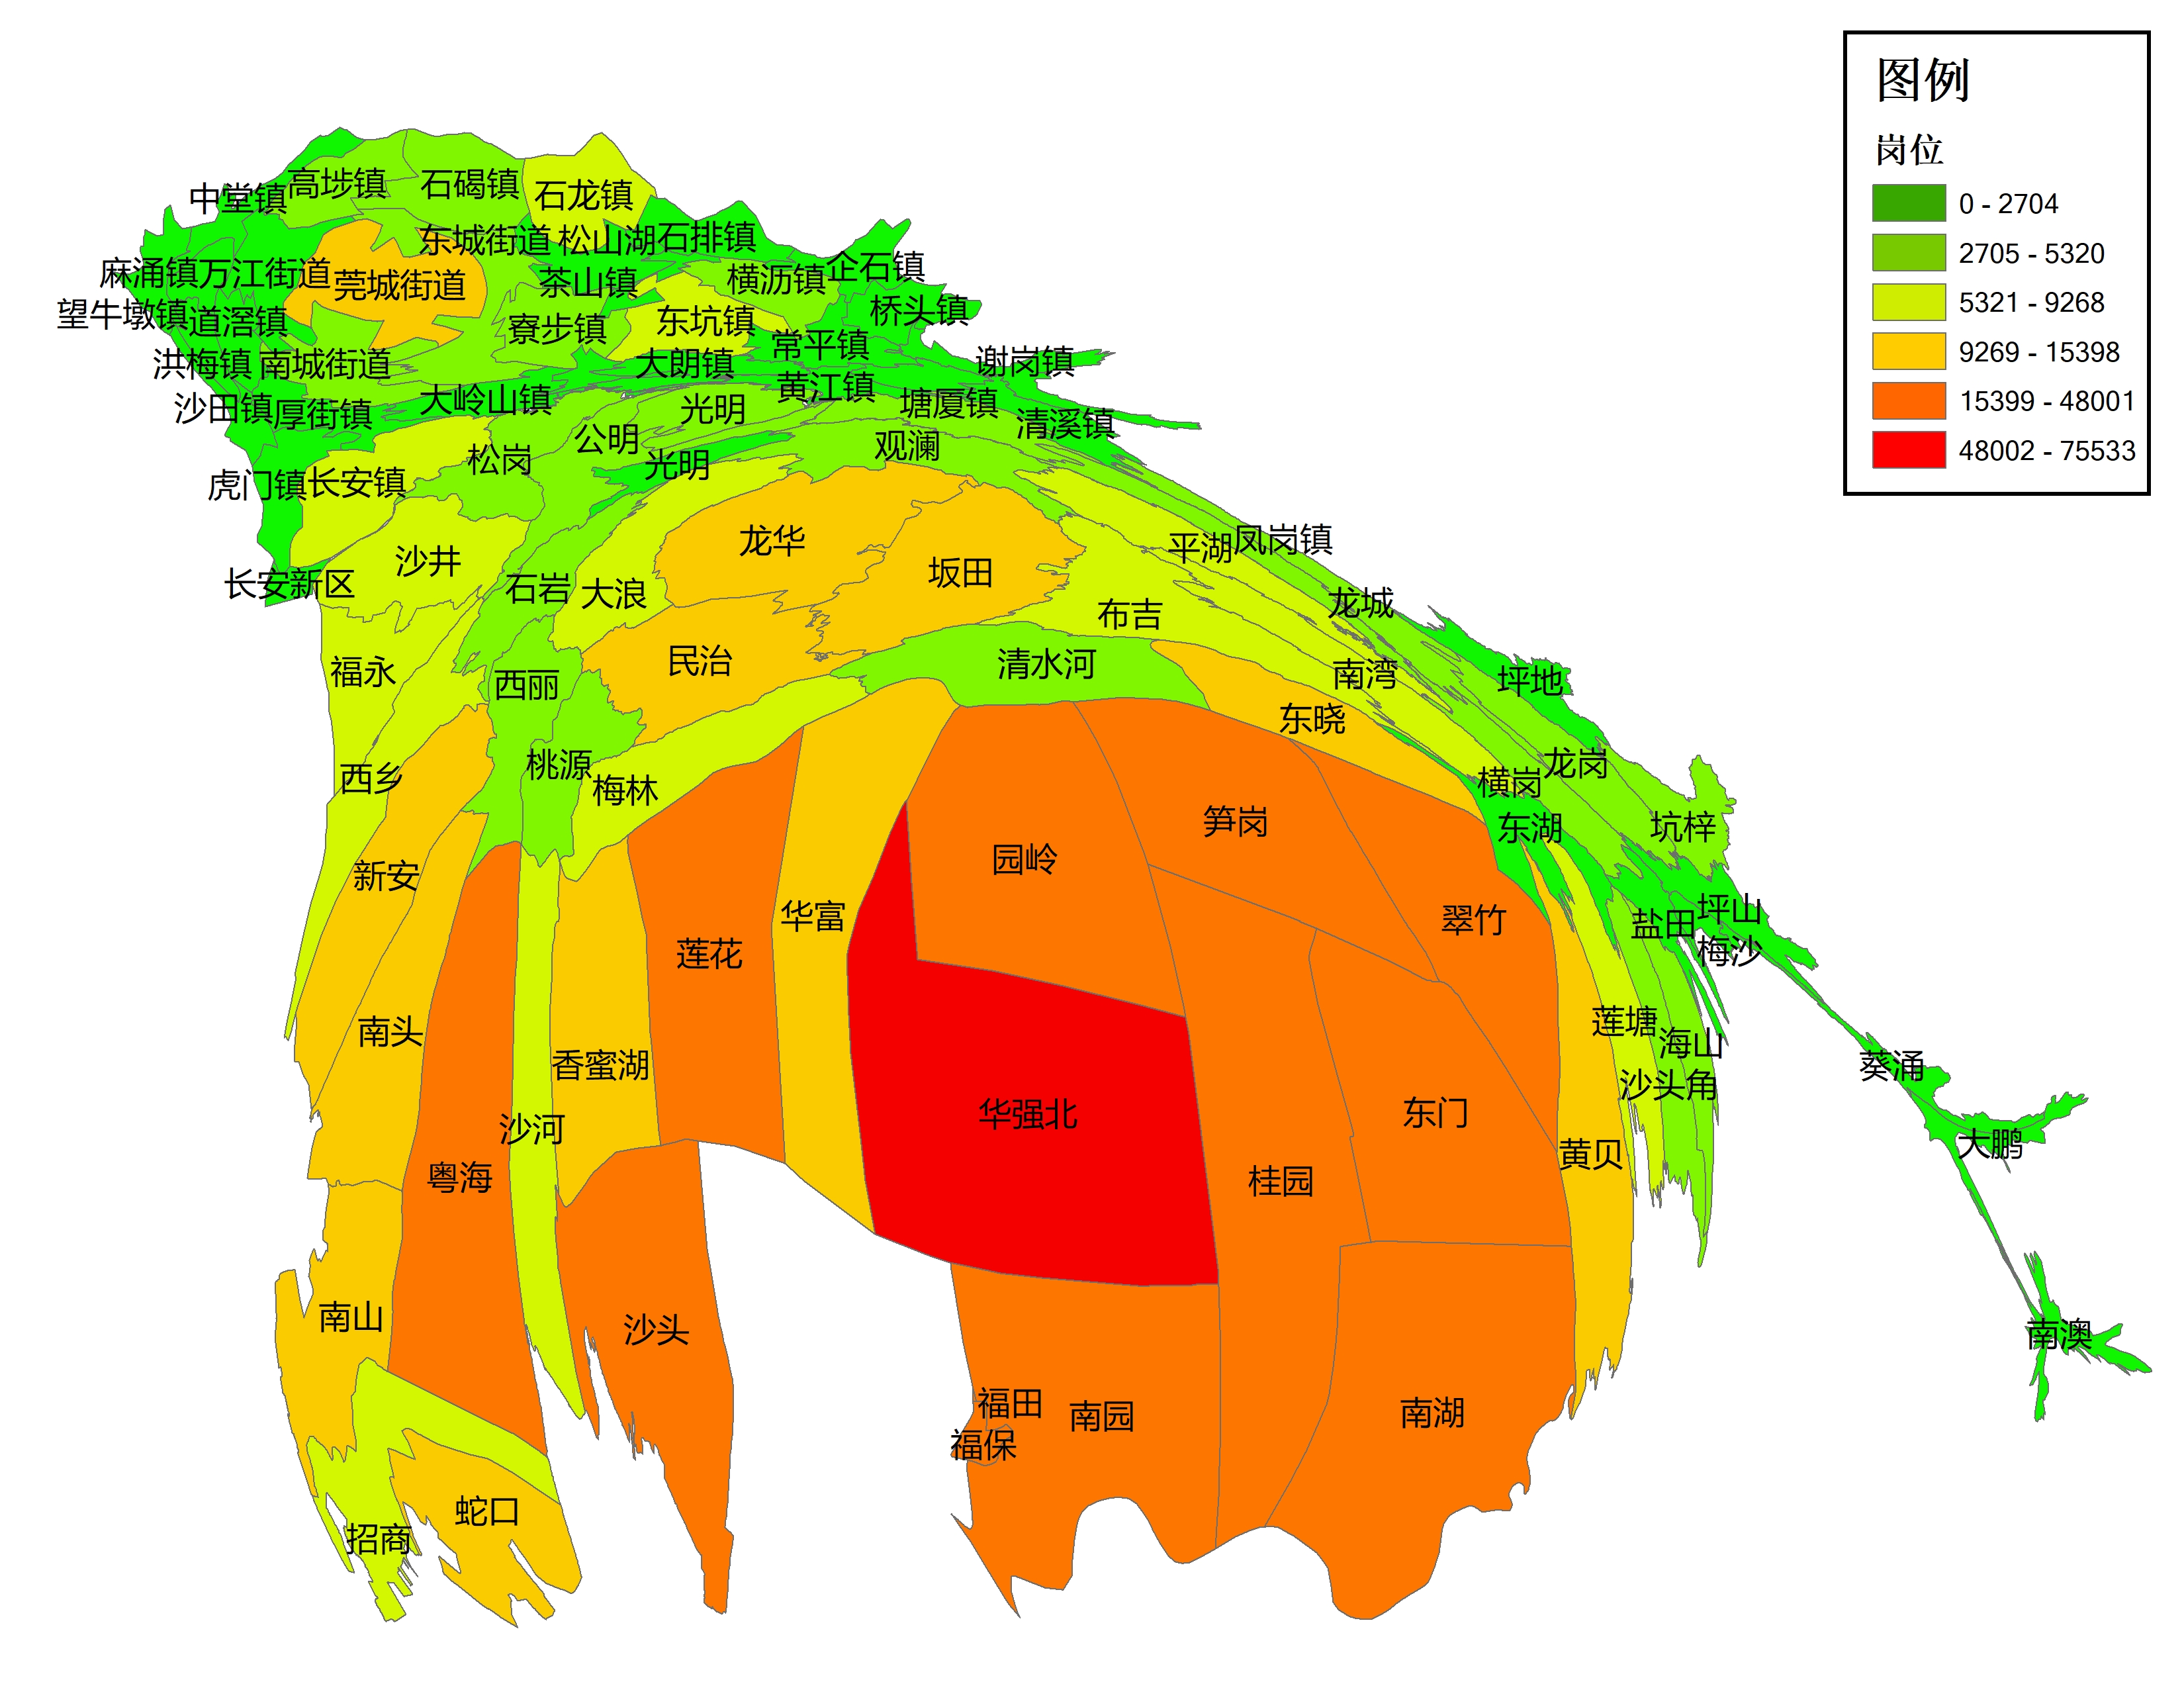
\includegraphics[width=0.7\textwidth]{chp04_岗位密度cartogram.jpg}
  \caption{深莞街道岗位密度变形地图(cartogram)}
\end{figure}
  \end{onlyenv}
%   \begin{onlyenv}<3>
% \begin{figure}[ht]
%   \centering
%   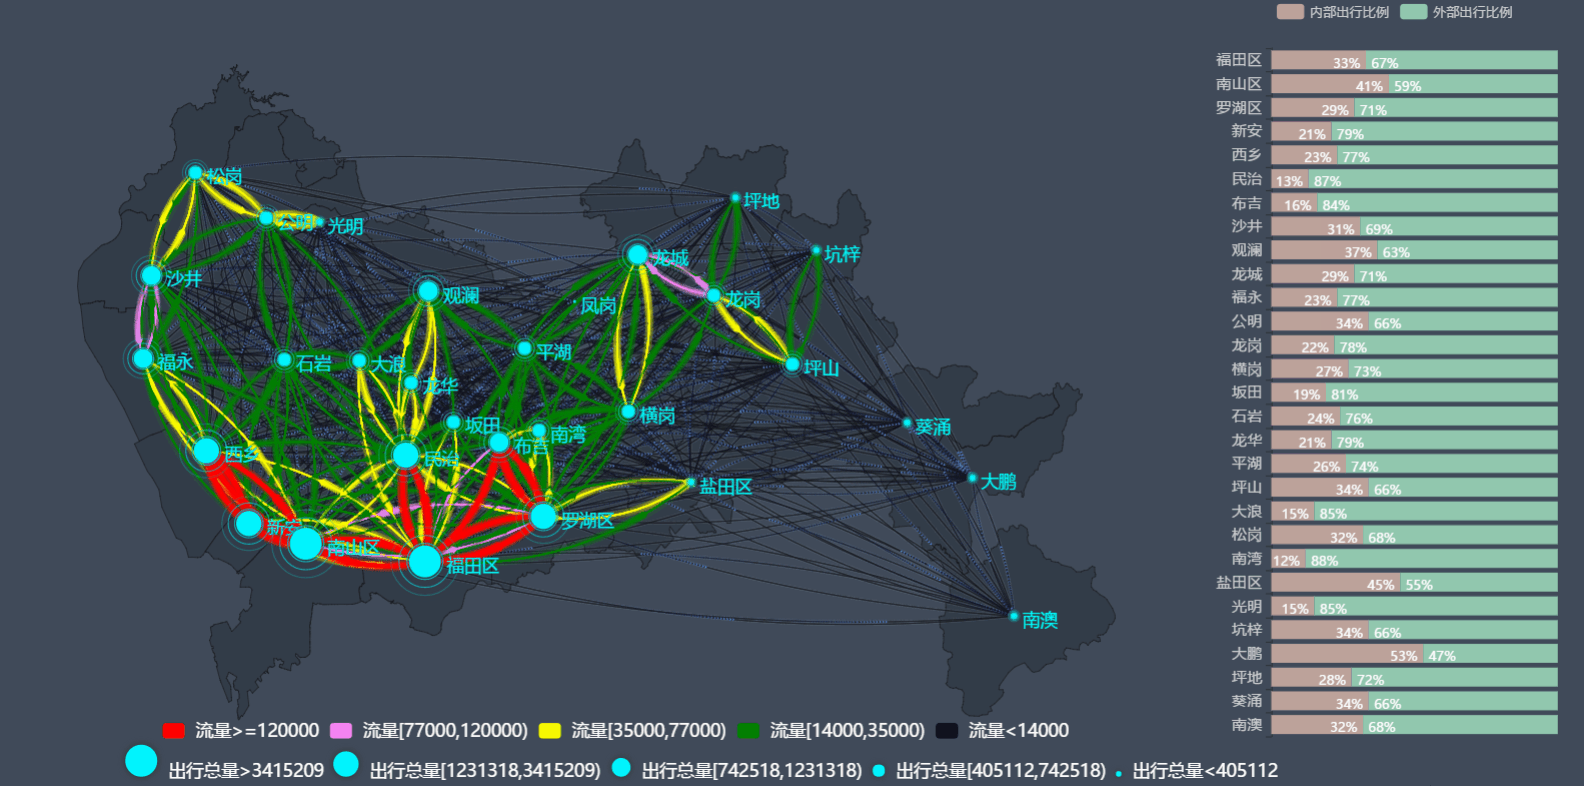
\includegraphics[width=\columnwidth]{chp03_流量可视化.png}
%   \caption{在一张图中同时展现总流量、OD量和内外部出行比例,数据在外部单独存储,与样式无关}
% \end{figure}
%   \end{onlyenv}
\end{overlayarea}
\end{frame}

\begin{frame}[t]{\subsecname}
\begin{itemize}
\item<1-> 计算机技术与艺术的结合
\item<2-> \emphText{将绘图与数据分离,数据相关绘图与数据无关绘图分离}
\item<3-> 示例:交通流量图
\end{itemize}

\begin{overlayarea}{\textwidth}{\textheight}
\vspace{-5pt}
  \begin{onlyenv}<3>
\begin{figure}[ht]
  \centering
  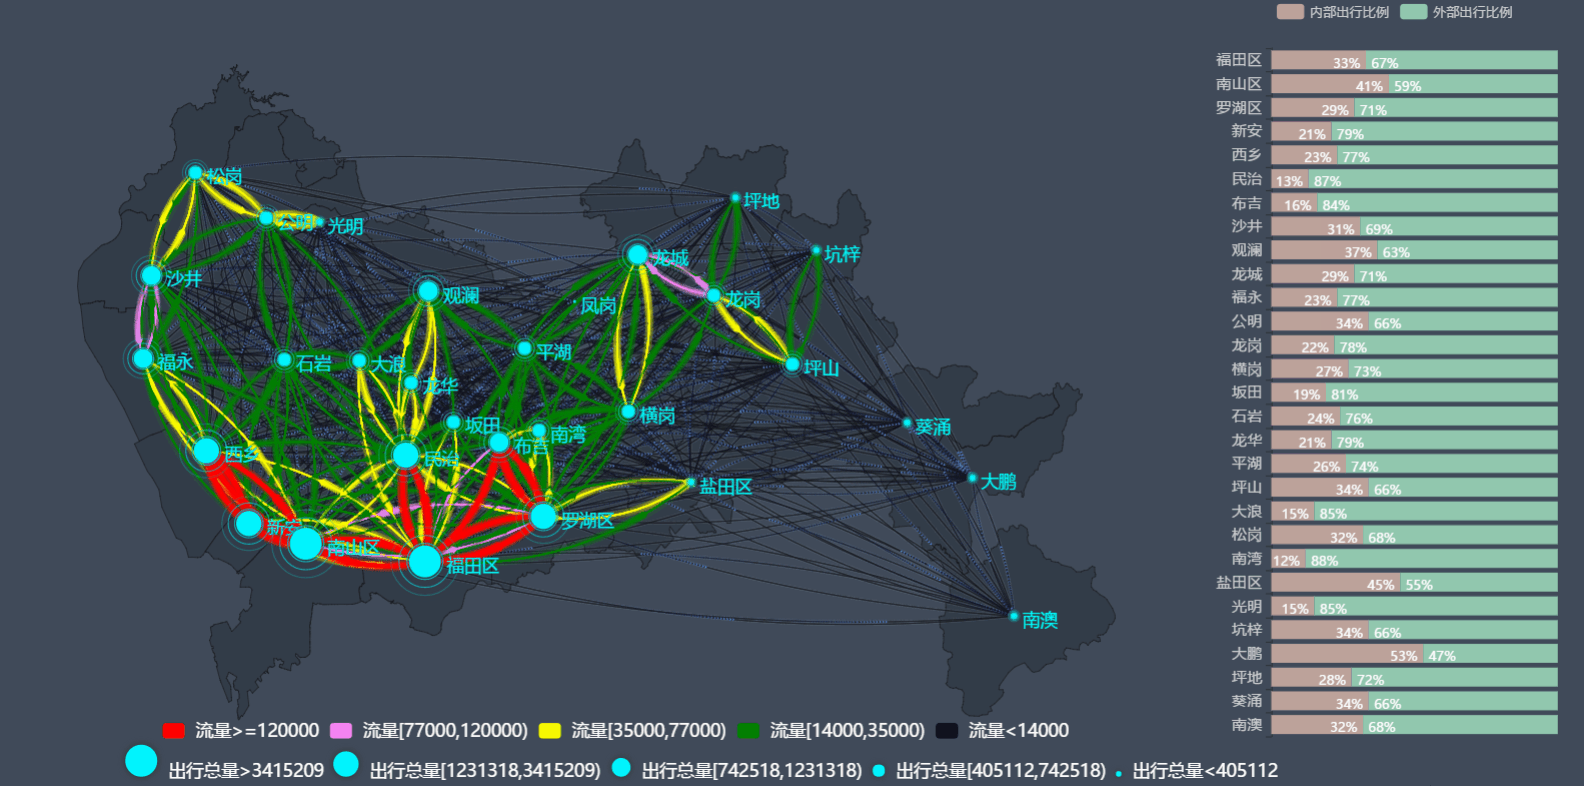
\includegraphics[width=\columnwidth]{chp03_流量可视化.png}
  \caption{在一张图中同时展现总流量、OD量和内外部出行比例,数据在外部单独存储,与样式无关}
\end{figure}
  \end{onlyenv}
\end{overlayarea}
\end{frame}

